%%%%%%%%%%%%%%%%%%%%%%%%%%%%%%%%%%%%%%%%%%%%%%%%%%%%%%%%%%%%%%%%%%%%%%
% Template for a UBC-compliant dissertation
% At the minimum, you will need to change the information found
% after the "Document meta-data"
%
%!TEX TS-program = pdflatex
%!TEX encoding = UTF-8 Unicode

%% The ubcdiss class provides several options:
%%   gpscopy (aka fogscopy)
%%       set parameters to exactly how GPS specifies
%%         * single-sided
%%         * page-numbering starts from title page
%%         * the lists of figures and tables have each entry prefixed
%%           with 'Figure' or 'Table'
%%       This can be tested by `\ifgpscopy ... \else ... \fi'
%%   10pt, 11pt, 12pt
%%       set default font size
%%   oneside, twoside
%%       whether to format for single-sided or double-sided printing
%%   balanced
%%       when double-sided, ensure page content is centred
%%       rather than slightly offset (the default)
%%   singlespacing, onehalfspacing, doublespacing
%%       set default inter-line text spacing; the ubcdiss class
%%       provides \textspacing to revert to this configured spacing
%%   draft
%%       disable more intensive processing, such as including
%%       graphics, etc.
%%

% For submission to GPS
\documentclass[gpscopy,onehalfspacing,11pt]{ubcdiss}
% For your own copies (looks nicer)
% \documentclass[balanced,twoside,11pt]{ubcdiss}

%%%%%%%%%%%%%%%%%%%%%%%%%%%%%%%%%%%%%%%%%%%%%%%%%%%%%%%%%%%%%%%%%%%%%%
%%%%%%%%%%%%%%%%%%%%%%%%%%%%%%%%%%%%%%%%%%%%%%%%%%%%%%%%%%%%%%%%%%%%%%
%%
%% FONTS:
%% 
%% The defaults below configures Times Roman for the serif font,
%% Helvetica for the sans serif font, and Courier for the
%% typewriter-style font.  Configuring fonts can be time
%% consuming; we recommend skipping to END FONTS!
%% 
%% If you're feeling brave, have lots of time, and wish to use one
%% your platform's native fonts, see the commented out bits below for
%% XeTeX/XeLaTeX.  This is not for the faint at heart. 
%% (And shouldn't you be writing? :-)
%%

%% NFSS font specification (New Font Selection Scheme)
\usepackage{times,mathptmx,courier}
\usepackage[scaled=.92]{helvet}

%% Math or theory people may want to include the handy AMS macros
\usepackage{amssymb} % for $\mathbb{R}$, Real R
%\usepackage{amsmath}
%\usepackage{amsfonts}

%% The pifont package provides access to the elements in the dingbat font.   
%% Use \ding{##} for a particular dingbat (see p7 of psnfss2e.pdf)
%%   Useful:
%%     51,52 different forms of a checkmark
%%     54,55,56 different forms of a cross (saltyre)
%%     172-181 are 1-10 in open circle (serif)
%%     182-191 are 1-10 black circle (serif)
%%     192-201 are 1-10 in open circle (sans serif)
%%     202-211 are 1-10 in black circle (sans serif)
%% \begin{dinglist}{##}\item... or dingautolist (which auto-increments)
%% to create a bullet list with the provided character.
\usepackage{pifont}

%%%%%%%%%%%%%%%%%%%%%%%%%%%%%%%%%%%%%%%%%%%%%%%%%%%%%%%%%%%%%%%%%%%%%%
%% Configure fonts for XeTeX / XeLaTeX using the fontspec package.
%% Be sure to check out the fontspec documentation.
%\usepackage{fontspec,xltxtra,xunicode}	% required
%\defaultfontfeatures{Mapping=tex-text}	% recommended
%% Minion Pro and Myriad Pro are shipped with some versions of
%% Adobe Reader.  Adobe representatives have commented that these
%% fonts can be used outside of Adobe Reader.
%\setromanfont[Numbers=OldStyle]{Minion Pro}
%\setsansfont[Numbers=OldStyle,Scale=MatchLowercase]{Myriad Pro}
%\setmonofont[Scale=MatchLowercase]{Andale Mono}

%% Other alternatives:
%\setromanfont[Mapping=tex-text]{Adobe Caslon}
%\setsansfont[Scale=MatchLowercase]{Gill Sans}
%\setsansfont[Scale=MatchLowercase,Mapping=tex-text]{Futura}
%\setmonofont[Scale=MatchLowercase]{Andale Mono}
%\newfontfamily{\SYM}[Scale=0.9]{Zapf Dingbats}
%% END FONTS
%%%%%%%%%%%%%%%%%%%%%%%%%%%%%%%%%%%%%%%%%%%%%%%%%%%%%%%%%%%%%%%%%%%%%%
%%%%%%%%%%%%%%%%%%%%%%%%%%%%%%%%%%%%%%%%%%%%%%%%%%%%%%%%%%%%%%%%%%%%%%



%%%%%%%%%%%%%%%%%%%%%%%%%%%%%%%%%%%%%%%%%%%%%%%%%%%%%%%%%%%%%%%%%%%%%%
%%%%%%%%%%%%%%%%%%%%%%%%%%%%%%%%%%%%%%%%%%%%%%%%%%%%%%%%%%%%%%%%%%%%%%
%%
%% Recommended packages
%%
\usepackage{checkend}	% better error messages on left-open environments
\usepackage{graphicx}	% for incorporating external images

%% booktabs: provides some special commands for typesetting tables as used
%% in excellent journals.  Ignore the examples in the Lamport book!
\usepackage{booktabs}

%% listings: useful support for including source code listings, with
%% optional special keyword formatting.  The \lstset{} causes
%% the text to be typeset in a smaller sans serif font, with
%% proportional spacing.
\usepackage{listings}
\lstset{basicstyle=\sffamily\scriptsize,showstringspaces=false,fontadjust}

%% The acronym package provides support for defining acronyms, providing
%% their expansion when first used, and building glossaries.  See the
%% example in glossary.tex and the example usage throughout the example
%% document.
%% NOTE: to use \MakeTextLowercase in the \acsfont command below,
%%   we *must* use the `nohyperlinks' option -- it causes errors with
%%   hyperref otherwise.  See Section 5.2 in the ``LaTeX 2e for Class
%%   and Package Writers Guide'' (clsguide.pdf) for details.
\usepackage[printonlyused,nohyperlinks]{acronym}
%% The ubcdiss.cls loads the `textcase' package which provides commands
%% for upper-casing and lower-casing text.  The following causes
%% the acronym package to typeset acronyms in small-caps
%% as recommended by Bringhurst.
\renewcommand{\acsfont}[1]{{\scshape \MakeTextLowercase{#1}}}

%% color: add support for expressing colour models.  Grey can be used
%% to great effect to emphasize other parts of a graphic or text.
%% For an excellent set of examples, see Tufte's "Visual Display of
%% Quantitative Information" or "Envisioning Information".
\usepackage{color}
\definecolor{greytext}{gray}{0.5}

%% comment: provides a new {comment} environment: all text inside the
%% environment is ignored.
%%   \begin{comment} ignored text ... \end{comment}
\usepackage{comment}

%% The natbib package provides more sophisticated citing commands
%% such as \citeauthor{} to provide the author names of a work,
%% \citet{} to produce an author-and-reference citation,
%% \citep{} to produce a parenthetical citation.
%% We use \citeeg{} to provide examples
\usepackage[numbers,sort&compress]{natbib}
\newcommand{\citeeg}[1]{\citep[e.g.,][]{#1}}

%% The titlesec package provides commands to vary how chapter and
%% section titles are typeset.  The following uses more compact
%% spacings above and below the title.  The titleformat that follow
%% ensure chapter/section titles are set in singlespace.
\usepackage[compact]{titlesec}
\titleformat*{\section}{\singlespacing\raggedright\bfseries\Large}
\titleformat*{\subsection}{\singlespacing\raggedright\bfseries\large}
\titleformat*{\subsubsection}{\singlespacing\raggedright\bfseries}
\titleformat*{\paragraph}{\singlespacing\raggedright\itshape}

%% The caption package provides support for varying how table and
%% figure captions are typeset.
\usepackage[format=hang,indention=-1cm,labelfont={bf},margin=1em]{caption}

%% url: for typesetting URLs and smart(er) hyphenation.
%% \url{http://...} 
\usepackage{url}
\urlstyle{sf}	% typeset urls in sans-serif


%%%%%%%%%%%%%%%%%%%%%%%%%%%%%%%%%%%%%%%%%%%%%%%%%%%%%%%%%%%%%%%%%%%%%%
%%%%%%%%%%%%%%%%%%%%%%%%%%%%%%%%%%%%%%%%%%%%%%%%%%%%%%%%%%%%%%%%%%%%%%
%%
%% Possibly useful packages: you may need to explicitly install
%% these from CTAN if they aren't part of your distribution;
%% teTeX seems to ship with a smaller base than MikTeX and MacTeX.
%%
%\usepackage{pdfpages}	% insert pages from other PDF files
%\usepackage{longtable}	% provide tables spanning multiple pages
%\usepackage{chngpage}	% support changing the page widths on demand
%\usepackage{tabularx}	% an enhanced tabular environment

%% enumitem: support pausing and resuming enumerate environments.
%\usepackage{enumitem}

%% rotating: provides two environments, sidewaystable and sidewaysfigure,
%% for typesetting tables and figures in landscape mode.  
%\usepackage{rotating}

%% subfig: provides for including subfigures within a figure,
%% and includes being able to separately reference the subfigures.
%\usepackage{subfig}

%% ragged2e: provides several new new commands \Centering, \RaggedLeft,
%% \RaggedRight and \justifying and new environments Center, FlushLeft,
%% FlushRight and justify, which set ragged text and are easily
%% configurable to allow hyphenation.
%\usepackage{ragged2e}

%% The ulem package provides a \sout{} for striking out text and
%% \xout for crossing out text.  The normalem and normalbf are
%% necessary as the package messes with the emphasis and bold fonts
%% otherwise.
%\usepackage[normalem,normalbf]{ulem}    % for \sout

%%%%%%%%%%%%%%%%%%%%%%%%%%%%%%%%%%%%%%%%%%%%%%%%%%%%%%%%%%%%%%%%%%%%%%
%% HYPERREF:
%% The hyperref package provides for embedding hyperlinks into your
%% document.  By default the table of contents, references, citations,
%% and footnotes are hyperlinked.
%%
%% Hyperref provides a very handy command for doing cross-references:
%% \autoref{}.  This is similar to \ref{} and \pageref{} except that
%% it automagically puts in the *type* of reference.  For example,
%% referencing a figure's label will put the text `Figure 3.4'.
%% And the text will be hyperlinked to the appropriate place in the
%% document.
%%
%% Generally hyperref should appear after most other packages

%% The following puts hyperlinks in very faint grey boxes.
%% The `pagebackref' causes the references in the bibliography to have
%% back-references to the citing page; `backref' puts the citing section
%% number.  See further below for other examples of using hyperref.
%% 2009/12/09: now use `linktocpage' (Jacek Kisynski): GPS now prefers
%%   that the ToC, LoF, LoT place the hyperlink on the page number,
%%   rather than the entry text.
\usepackage[bookmarks,bookmarksnumbered,%
    allbordercolors={0.8 0.8 0.8},%
    pagebackref,linktocpage%
    ]{hyperref}
%% The following change how the the back-references text is typeset in a
%% bibliography when `backref' or `pagebackref' are used
\renewcommand\backrefpagesname{\(\rightarrow\) pages}
\renewcommand\backref{\textcolor{greytext} \backrefpagesname\ }

%% The following uses most defaults, which causes hyperlinks to be
%% surrounded by colourful boxes; the colours are only visible in
%% PDFs and don't show up when printed:
%\usepackage[bookmarks,bookmarksnumbered]{hyperref}

%% The following disables the colourful boxes around hyperlinks.
%\usepackage[bookmarks,bookmarksnumbered,pdfborder={0 0 0}]{hyperref}

%% The following disables all hyperlinking, but still enabled use of
%% \autoref{}
%\usepackage[draft]{hyperref}

%% The following commands causes chapter and section references to
%% uppercase the part name.
\renewcommand{\chapterautorefname}{Chapter}
\renewcommand{\sectionautorefname}{Section}
\renewcommand{\subsectionautorefname}{Section}
\renewcommand{\subsubsectionautorefname}{Section}

%% If you have long page numbers (e.g., roman numbers in the 
%% preliminary pages for page 28 = xxviii), you might need to
%% uncomment the following and tweak the \@pnumwidth length
%% (default: 1.55em).  See the tocloft documentation at
%% http://www.ctan.org/tex-archive/macros/latex/contrib/tocloft/
% \makeatletter
% \renewcommand{\@pnumwidth}{3em}
% \makeatother

%%%%%%%%%%%%%%%%%%%%%%%%%%%%%%%%%%%%%%%%%%%%%%%%%%%%%%%%%%%%%%%%%%%%%%
%%%%%%%%%%%%%%%%%%%%%%%%%%%%%%%%%%%%%%%%%%%%%%%%%%%%%%%%%%%%%%%%%%%%%%
%%
%% Some special settings that controls how text is typeset
%%
% \raggedbottom		% pages don't have to line up nicely on the last line
% \sloppy		% be a bit more relaxed in inter-word spacing
% \clubpenalty=10000	% try harder to avoid orphans
% \widowpenalty=10000	% try harder to avoid widows
% \tolerance=1000


%%%%%%%%%%%%%%%%%%%%%%%%%%%%%%%%%%%%%%%%%%%%%%%%%%%%%%%%%%%%%%%%%%%%%%
%%%%%%%%%%%%%%%%%%%%%%%%%%%%%%%%%%%%%%%%%%%%%%%%%%%%%%%%%%%%%%%%%%%%%%
%%
%% Document meta-data: be sure to also change the \hypersetup information
%%

\title{Master's Thesis Draft}
%\subtitle{If you want a subtitle}

\author{Victor Gan}
\previousdegree{BSc, University of Waterloo, 2013}

% What is this dissertation for?
\degreetitle{Master of Science}

\institution{The University of British Columbia}
\campus{Vancouver}

\faculty{The Faculty of Science}
\department{Computer Science}
\submissionmonth{April}
\submissionyear{2015}

%% hyperref package provides support for embedding meta-data in .PDF
%% files
\hypersetup{
  pdftitle={Change this title!  (DRAFT: \today)},
  pdfauthor={Victor Gan},
  pdfkeywords={Your keywords here}
}

%%%%%%%%%%%%%%%%%%%%%%%%%%%%%%%%%%%%%%%%%%%%%%%%%%%%%%%%%%%%%%%%%%%%%%
%%%%%%%%%%%%%%%%%%%%%%%%%%%%%%%%%%%%%%%%%%%%%%%%%%%%%%%%%%%%%%%%%%%%%%
%% 
%% The document content
%%



%%%%%%%%%%%%%%%%%%%%%%%%%%%%%%%%%%%%%%%%%%%%%%%%%%
%% From Thesis Components: Tradtional Thesis
%% <http://www.grad.ubc.ca/current-students/dissertation-thesis-preparation/order-components>

\usepackage{csquotes} % For \blockquote
\usepackage[chapter]{algorithm} % chapter makes numbering relative to chapter
\usepackage{algpseudocode}
\algrenewcommand\algorithmicrequire{\textbf{Precondition:}}
\algrenewcommand\algorithmicensure{\textbf{Postcondition:}}


\input{macros} % Template's macros

% \includeonly to limit which \include{}'s to insert
% \includeonly{contents/intro, contents/method}
\begin{document}

% ====================
% Preliminary Pages (numbered in lower case Roman numerals)
% ====================

%    1. Title page (mandatory)
\maketitle

%    2. Abstract (mandatory - maximum 350 words)
%% The following is a directive for TeXShop to indicate the main file
%%!TEX root = diss.tex

\chapter{Abstract}

This document provides brief instructions for using the \class{ubcdiss}
class to write a \acs{UBC}-conformant dissertation in \LaTeX.  This
document is itself written using the \class{ubcdiss} class and is
intended to serve as an example of writing a dissertation in \LaTeX.
This document has embedded \acp{URL} and is intended to be viewed
using a computer-based \ac{PDF} reader.

Note: Abstracts should generally try to avoid using acronyms.

Note: at \ac{UBC}, both the \ac{GPS} Ph.D. defence programme and the
Library's online submission system restricts abstracts to 350
words.

% Consider placing version information if you circulate multiple drafts
%\vfill
%\begin{center}
%\begin{sf}
%\fbox{Revision: \today}
%\end{sf}
%\end{center}

\cleardoublepage

%    3. Preface
%% The following is a directive for TeXShop to indicate the main file
%%!TEX root = diss.tex

\chapter{Preface}

At \ac{UBC}, a preface may be required.  Be sure to check the
\ac{GPS} guidelines as they may have specific content to be included.

\cleardoublepage
% 
%    4. Table of contents (mandatory - list all items in the preliminary pages
%    starting with the abstract, followed by chapter headings an

%    subheadings, bibliographies and appendices)
\tableofcontents
\cleardoublepage	% required by tocloft package

%    5. List of tables (mandatory if thesis has tables)
\listoftables
\cleardoublepage	% required by tocloft package

%    6. List of figures (mandatory if thesis has figures)
\listoffigures
\cleardoublepage	% required by tocloft package

\listofalgorithms
\addcontentsline{toc}{chapter}{List of Algorithms}
\cleardoublepage	% required by tocloft package
 
 %    7. List of illustrations (mandatory if thesis has illustrations)
 %    8. Lists of symbols, abbreviations or other (optional)
 
 %    9. Glossary (optional)
 %% The following is a directive for TeXShop to indicate the main file
%%!TEX root = diss.tex

\chapter{Glossary}

This glossary uses the handy \latexpackage{acroynym} package to automatically
maintain the glossary.  It uses the package's \texttt{printonlyused}
option to include only those acronyms explicitly referenced in the
\LaTeX\ source.

% use \acrodef to define an acronym, but no listing
\acrodef{UI}{user interface}
\acrodef{UBC}{University of British Columbia}

% The acronym environment will typeset only those acronyms that were
% *actually used* in the course of the document
\begin{acronym}[ANOVA]
\acro{ANOVA}[ANOVA]{Analysis of Variance\acroextra{, a set of
  statistical techniques to identify sources of variability between groups}}
\acro{API}{application programming interface}
\acro{CTAN}{\acroextra{The }Common \TeX\ Archive Network}
\acro{DOI}{Document Object Identifier\acroextra{ (see
    \url{http://doi.org})}}
\acro{GPS}[GPS]{Graduate and Postdoctoral Studies}
\acro{PDF}{Portable Document Format}
\acro{RCS}[RCS]{Revision control system\acroextra{, a software
    tool for tracking changes to a set of files}}
\acro{TLX}[TLX]{Task Load Index\acroextra{, an instrument for gauging
  the subjective mental workload experienced by a human in performing
  a task}}
\acro{UML}{Unified Modelling Language\acroextra{, a visual language
    for modelling the structure of software artefacts}}
\acro{URL}{Unique Resource Locator\acroextra{, used to describe a
    means for obtaining some resource on the world wide web}}
\acro{W3C}[W3C]{\acroextra{the }World Wide Web Consortium\acroextra{,
    the standards body for web technologies}}
\acro{XML}{Extensible Markup Language}
\end{acronym}

% You can also use \newacro{}{} to only define acronyms
% but without explictly creating a glossary
% 
% \newacro{ANOVA}[ANOVA]{Analysis of Variance\acroextra{, a set of
%   statistical techniques to identify sources of variability between groups.}}
% \newacro{API}[API]{application programming interface}
% \newacro{GOMS}[GOMS]{Goals, Operators, Methods, and Selection\acroextra{,
%   a framework for usability analysis.}}
% \newacro{TLX}[TLX]{Task Load Index\acroextra{, an instrument for gauging
%   the subjective mental workload experienced by a human in performing
%   a task.}}
% \newacro{UI}[UI]{user interface}
% \newacro{UML}[UML]{Unified Modelling Language}
% \newacro{W3C}[W3C]{World Wide Web Consortium}
% \newacro{XML}[XML]{Extensible Markup Language}
	% always input, since other macros may rely on it
 
 \textspacing		% begin one-half or double spacing
 
 %   10. Acknowledgements (optional)
 %% The following is a directive for TeXShop to indicate the main file
%%!TEX root = diss.tex

\chapter{Acknowledgments}

Thank those people who helped you. 

Don't forget your parents or loved ones.

You may wish to acknowledge your funding sources.

NSERC CGS-M scholarship.


Julieta Martinez for the discussions.

 
 %   11. Dedication (optional)

% ====================
% Body of Thesis (not all sections may apply)
\mainmatter
\acresetall	% reset all acronyms used so far
% ====================

% --------------------
%    1. Introduction
% --------------------
%% The following is a directive for TeXShop to indicate the main file
%%!TEX root = diss.tex

% Describe the problem
% State your contributions (write the list of contributions fist)
% that’s all
% use an example to introduce the problem
% Reader thinks“gosh, if they can really deliver this, that’d be exciting; Id
% bet- ter read on” [? ]
% Contributions should be refutable
% No ”the rest of the paper is”. Instead, use forward references from the nar-
% rative in the introduction. The introduction (including the contributions)
% should survey the whole paper, and therefore forward reference every im-
% portant part

\chapter{Introduction}
\label{ch:Introduction}





% Purpose: Motivate the need of an autonomous back-in parking system.

% Lack of mobility leads to social, psychological and physical problems.
Mobility impairment is a significant problem for older adults. Mobility is
shown to be pivotal to the quality of life of residents in long-term care
facilities, offering a means of freedom, choice and independence
\cite{bourret2002meaning}.

% The potential impact for smart wheelchairs is significant.
Smart wheelchairs have a large potential for impact.
One method in aiding mobility is using powered wheelchairs with additional smart
capabilities.
An estimated 1.4 million to 2.1 million individuals in the US in 2008 stood to
benefit from smart wheelchairs, and an estimated 973 thousand to 1.7 million of
those stood to benefit from autonomous navigation capabilities in particular.
These estimates are expected to grow proportional to the increase in
wheelchair users, which grows at a rate of 5.9 percent per year
\cite{simpson2008many}.

% Smart wheelchairs are needed.
However, it may be impossible for persons with severe disabilities to maneuver PWCs
given their current control interfaces: 10\% of patients who receive PWC training
find it extremely difficult or impossible to use the wheelchair for activities of
daily living \cite{fehr2000adequacy}.
Moreso, when asked specifically about steering and maneuvering tasks, the
percentage of patients reported to find these difficult or impossible jumped to
40\%, and nearly half of patients unable to control a power wheelchair by
conventional methods would benefit from an automated navigation system.
Due to this, Fehr et al. \cite{fehr2000adequacy} concludes supervised autonomous
navigation is necessary over improved steering interfaces.

% Semi-automation is the way to go
Though autonomous tasks are necessary, total autonomy is hard and may not even be desired. 
A totally autonomous system may deprive user's feeling of being in control 
\cite{viswanathana2014wizard}.
Older adults preferred robot assistance over human assistance for tasks related
to chores, manipulating objects, and information management, but not personal
care and leisure activities \cite{smarr2014domestic}.
Instead, systems that complete specific chore-like tasks akin to automatic
parallel parking or cruise control on a car is more suitable.

% There has been some progress on semi-automation
This leads to the need of task-specific autonomous behaviours.
Some work has been done on task-specific autonomous PWC behaviours, including
navigation in crowded environments \cite{prassler2001robotics}, obstacle
avoidance \cite{viswanathan2012navigation}, and docking onto lift platforms
\cite{sermeno2006vision} and custom-designed beds \cite{ren2012docking}.
More general overviews of smart wheelchair systems can be found in
\cite{viswanathan2012navigation, simpson2005smart, faria2013patient} (TODO
confirm).

% Not much in general back-in parking, a very common task in the target demographic
Little work has been done to dock/back-in park a wheelchair in a more general
environment, such a general indoor office environment akin to a room in a
long-term care facility. 


% Done: Bikram's thesis intro, Pouria's thesis intro

On

% TODO talk about shared control? Pouria's thesis, page 1

\section{Previous work on Smart Wheelchairs}

\section{Hardware}
We use a (TODO model) by (TODO) 

We use a Lenovo W530 laptop with 
\begin{itemize}
\item Intel Core i7-3720QM Processor
\item 8GB RAM
\item 120GB SSD
\item NVIDIA Quadro K1000M Graphical Processing Unit
\item Two dedicated USB controllers for USB 2.0 and USB 3.0
\item Ubuntu 14.04 64-bit
\item Robotic Operating System (Indigo release)
\end{itemize}

(Contributions) In this paper we put this point on a further basis:
\begin{itemize}
\item contribution 1
\end{itemize}

% ======================
\endinput
Any text after an \endinput is ignored.
% ======================

% ====================
\section{Summary of Thesis}
% ====================
% --------------------
\subsection{One sentence summary}
% --------------------
We introduce an autonomous back-in parking system for powered wheelchairs
equipped with an RGB-D sensor.

% --------------------
\subsection{One paragraph summary}
% --------------------

% --------------------
\subsection{Five minute read summary}
% --------------------

\paragraph{What is this?} A collection of research ideas.

\paragraph{Who's it for?} Me.

TODO use this \cite{viswanathan2011navigation}


% --------------------
%    2. Main body
% --------------------

% --------------------
% % ====================
\chapter{The Problem}
% ====================

% ====================
\section{Problem Goals}
% ====================
% \begin{itemize}
% \item Advances scientific understanding of the world
% \item Be general enough to be widely useful
% \item Novel: don't work on things everyone else is.
% \end{itemize}

% ====================
\section{Specific Problem}
% ====================



% --------------------

% --------------------
% ===================================================
\chapter{Background}
% ===================================================


% ===================================================
\section{Notation for Traditional Path Planning}
% ===================================================

[TODO avoid definition notation]
\theoremstyle{definition}
\begin{definition}{Maximal Reachable Set}
A fibration is a mapping between two topological spaces that has the homotopy lifting property for every space $X$.
\end{definition}

Taken from page 17 of \cite{lavalle2006planning}:

\begin{definition}{State}
Temp
\end{definition}

\begin{definition}{state space $X$}
Finite or countably infinite set of states.
\end{definition}

\begin{definition}{Initial State $x_1 \in X$}
Temp
\end{definition}

\begin{definition}{Goal Set $X_G \subset X$}
Temp
\end{definition}

\begin{definition}{Time}
Temp
\end{definition}

\begin{definition}{Action $u$}
Temp
\end{definition}

\begin{definition}{action space $U(x)$}
A finite set of actions for each state $x \in X$
\end{definition}

\begin{definition}{(state transition function)}
 $f(x,u) \in X$
A finite set of actions for each state $x \in X$
\end{definition}

\begin{definition}{Feasibility Criterion}
Temp
\end{definition}

\begin{definition}{Optimality Criterion}
Temp
\end{definition}

\begin{definition}{Plan}
Temp
\end{definition}

\begin{definition}{Potential Function}
Temp
\end{definition}

\begin{definition}{Configuration Space}
Temp
\end{definition}

\begin{definition}{XYZ Space}
Temp
\end{definition}

\begin{definition}{XY Space $M$}
Temp
\end{definition}

% ===================================================
\chapter{Related Work}
% ===================================================
% show my problem is unsolved
% • show my problem is interesting
% • show my idea works
% • show how my idea compares to other ideas
% • No related work yet! Include at end.
% – Problem 1: describing alternative approaches gets between the reader
% and your idea (I feel tired)
% – Problem 2: the reader knows nothing about the problem yet; so your
% (carefully trimmed) description of various technical tradeoffs is abso-
% lutely incomprehensible (I feel stupid)
% – instead, Concentrate single-mindedly on a narrative that
% ∗ Describes the problem, and why it is interesting
% ∗ Describes your idea
% ∗ Defends your idea, showing how it solves the problem, and filling
% out the details
% ∗ On the way, cite relevant work in passing, but defer discussion to
% the end
% • show how my idea compares to other ideas
% • Be generous to the competition. In his inspiring paper [Foo98] Foogle shows....
% We develop his foundation in the following ways...
% • Giving credit to others does not diminish the credit you get from your paper
% • Acknowledge weaknesses in your approach
% • Failing to give credit to others can kill your paper: You don’t know that it’s
% an old idea (bad) or You do know, but are pretending it’s yours (very bad)

% ====================
\section{Parking Lot Detection}
% ====================
% Wang \cite{wang2014automatic}
% Jung \cite{jung2014semiautomatic}
% 
% Pouria's thesis \cite{talebifard2014risk}
% Talk: \url{https://www.youtube.com/watch?v=Db7EhLYf-Yk#t=1h11m07s}
% 
% 
% file:papers/jiang1999sensor.pdf
% Basic old paper on parallel parking. Uses ultrasonic sensor, then
% fixed planning.
% 
% file:papers/fairus2011development.pdf
% Old paper. Scanning methods.
% 
% file:papers/wang2013automatic.pdf
% Newish lit review of automatic parking
% 
% file:papers/abad2007parking.pdf
% Parking space detection using 3d vision. Parallel parking
% 
% file:papers/lalonde2012single.pdf
% CVPR workshop paper.
% 
% file:papers/suhr2010automatic.pdf
% Good! Solving my problem, but with a laser rangefinder.
% found from: http://www.mathworks.com/matlabcentral/answers/126413-how-to-detect-free-spots-in-a-parking-area
% 
% file:assets/WheelchairGuide.pdf

% ====================
\section{SLAM}
% ====================

LSD-Slam and PTAM for monocular seem to be state-of-art: \url{http://vision.in.tum.de/research/lsdslam}

review paper: \url{http://www-personal.acfr.usyd.edu.au/tbailey/papers/slamtute2.pdf}

2009 review paper: \url{http://www.le2i.cnrs.fr/IMG/publications/2172_Muhammad_EI_2009.pdf}

% ====================
\section{Collision Avoidance}
% ====================
Old paper using quadtrees\cite{ghoshray1996comprehensive}

Bigdog \cite{raibert2008bigdog}

Springer handbook of robotics \cite{siciliano2008springer}: Vector field histograms, as described in Pouria's thesis \cite{talebifard2014risk}


% ====================
\section{Time Optimal Trajectory Planning}
% ====================
\cite{fiorini1996time}

\section{Hardware}

[TODO photo]

We choose and fix the hardware used beforehand.

We use an RGB-D sensor due to its suitability to the problem:
it works well indoors, where the target users will be using the wheelchairs; it
is cost effective; it provides depth information with adequate accuracy.

We use only one camera. This is for simplicity. Each camera saturates its USB
controller, hence a computer must have as many USB controllers as cameras.
An additional calibration step to register the information, increasing the
computational costs even further than the linear factor. 
One can argue a limitation of using one RGB-D sensor is the depth measurements
have a range of around 0.6 m to 8 m, with a field of view of 43 degrees
vertically by 57 degrees horizontally (TODO better reference) \cite{endres2014catadioptric},
comparatively limited to lidars with fields of view of 180 degrees. Some work
\cite{endres2014catadioptric} has been done using two mirrors to split the field
of view of a single camera to cover both the front and rear view. Our work
sticks to a single camera for simplicity, though it can be naturally extended.

We mount the RGB-D camera downwards. However, we do not rely on a specific angle
to keep the solutions generalizable to systems that might have different camera
angles. The only assumption is the ground plane is visible.

We use an Asus RGB-D camera as it is smaller and less obtrusive than the Kinect
and does not require an additional power plug; it gets its power entirely from
USB.


We use a (TODO model) by (TODO) 

We use a Lenovo W530 laptop with 
\begin{itemize}
\item Intel Core i7-3720QM Processor
\item 8GB RAM
\item 120GB SSD
\item NVIDIA Quadro K1000M Graphical Processing Unit
\item Two dedicated USB controllers for USB 2.0 and USB 3.0
\item Ubuntu 14.04 64-bit
\item Robotic Operating System (Indigo release)
\end{itemize}

% ======================
\endinput
Any text after an \endinput is ignored.
% ======================
% ===================================================
\section{Robotics Pipelines}
% ===================================================

% ---------------------------------------------------
\subsection{Robotic Operating System}
% ---------------------------------------------------

% ---------------------------------------------------
\subsection{Robotic Operating System}
% ---------------------------------------------------

% ===================================================
\section{Modeling}
% ===================================================

% ---------------------------------------------------
\subsection{Classification}
% ---------------------------------------------------
Modeling 

% ---------------------------------------------------
\subsection{Bayesian Stuff}
% ---------------------------------------------------
Chiu-Liu Trees

% ---------------------------------------------------
\subsection{Markov Chains, MDPs, POMDPs}
% ---------------------------------------------------

% ---------------------------------------------------
\subsection{Reinforcement Learning}
% ---------------------------------------------------
Value function, reward function

% ---------------------------------------------------
\subsection{Path Planning}
% ---------------------------------------------------

% ---------------------------------------------------
\subsection{Bandit Problems}
% ---------------------------------------------------

% ---------------------------------------------------
\subsection{Feasibility}
% ---------------------------------------------------

% ---------------------------------------------------
\subsection{Game Theory}
% ---------------------------------------------------

% ---------------------------------------------------
\subsection{Control}
% ---------------------------------------------------

% ---------------------------------------------------
\subsection{Rotations}
% ---------------------------------------------------

% ---------------------------------------------------
\subsection{Distance Transforms and Geodesics}
% ---------------------------------------------------

% ---------------------------------------------------
\subsection{Visual Servoing}
% ---------------------------------------------------
% https://en.wikipedia.org/wiki/Visual_servoing

% --------------------

% --------------------
% ====================
\chapter{Method (My Idea)}
% ====================

% • In a paper you MUST provide the details, but FIRST convey the idea
% • Introduce the problem, and your idea, using EXAMPLES and only then
% present the general case
% • Explain it as if you were speaking to someone using a whiteboard
% • Conveying the intuition is primary, not secondary
% • Once your reader has the intuition, she can follow the details (but not vice
% versa)
% Even if she skips the details, she still takes away something valuable
% Evidence
% • Your introduction makes claims; The body of the paper provides evidence to
% support each claim
% • Check each claim in the introduction, identify the evidence, and forward-
% reference it from the claim
% • Evidence can be: analysis and comparison, theorems, measurements, case
% studies

% ====================
\section{My Idea (2 pages)}
% ====================

% ====================
\section{The details (5 pages)}
% ====================

% ====================
\chapter{Motion Planning}
% ====================
% --------------------
\section{Basic Ingredients}
% --------------------
\begin{itemize}
\item State
\item Time
\item Actions
\item Initial and Goal States
\item Feasibility and Optimality Criterion
\item A Plan
\end{itemize}

For a full description, see Chapter 1.3 of Lavalle \cite{lavalle2006planning}.
% --------------------
\section{Introduction to Motion Planning}
% --------------------
% --------------------
\subsection{Simple Motion Planning}
% --------------------
The simplest motion planning problems assume knowledge of a global map, a fixed
known goal state and a fixed known initial state. The problem is to determine a
feasible path from the initial state to the goal state. An optimality criterion
may also be applied to choose the best path if multiple feasible ones are found.

Notably, two important concepts have often been ignored in determining the path:
the dynamics of the system and the use of feedback. Dynamics refers to how
states transition to other states, and is inherent in real-world systems. For
example, a car can easily move fowards and backwards, but cannot immediately
move side to side. Feedback refers to the technique of refining further actions
based on newly sensed data. In simulations, feedback may not be necessary, but
in real-world systems, errors in sensing and modeling build up over time without
it.

In this simple case, the generated path is followed in an open-loop manner, or
if subject to real-world constraints (see \autoref{fig:lavalle2006planning119}),
the generated path is smoothed to obey the system's dynamics and feedback is
used to closely follow the path. "Notably this approach is highly decoupled as
feedback and dynamics are neglected in constructing the original path"
\cite{lavalle2006planning}. The smooth path may now obey the robot's dynamics,
but may no longer be feasible.  Feedback is used merely as an inefficient
afterthought.

\begin{figure}
\centering
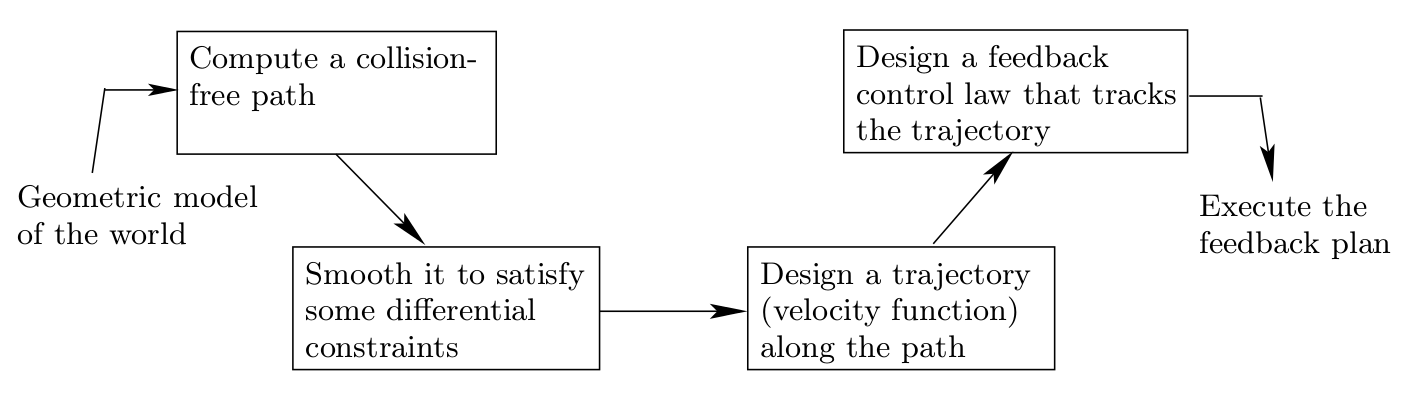
\includegraphics[width=3in]{figures/lavalle2006planning119.png}
\caption{From \cite{lavalle2006planning}. A refinement approach that has been used for decades in robotics.}
\label{fig:lavalle2006planning119}
\end{figure}

Even in this simple case, obtaining an optimal or even feasible path is not
straightforward if the state space is large. A* search for trivially sized state
spaces and sampling-based techniques such as RRTs (RRT* for optimality) and PRMs
have proven to be the methods of choice (citation?), though it is still an
ongoing field of interest (cite 2015 RRT/PRM papers).

% --------------------
\subsection{Feedback Motion Planning}
% --------------------
Dynamics refers, generally, to how a state transitions to another state.

Feedback (or reactive plans) refers to something else.

Tiers of motion planning problems
\begin{itemize}
\item Fixed Initial and Goal States, no dynamics, no feedback, some optimality
criterion: RRT*, PRM*
\item Fixed Initial and Goal States, dynamics, no feedback: RRT*, A*
\item Fixed Initial and Goal States, no dynamics, feedback
\end{itemize}

see \autoref{fig:determinedrive2}.
\begin{figure}
\centering
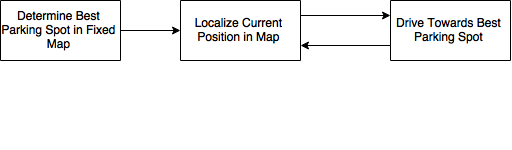
\includegraphics[width=3in]{figures/determinedrive2.png}
\caption{Feedback loop}
\label{fig:determinedrive2}
\end{figure}


% --------------------
\subsection{Feedback Motion Planning with Updating Goal State}
% --------------------
see \autoref{fig:determinedrive1}.
For a full description, see Chapter 8 of Lavalle \cite{lavalle2006planning}.

\begin{figure}
\centering
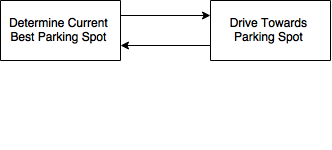
\includegraphics[width=3in]{figures/determinedrive1.png}
\caption{Feedback loop}
\label{fig:determinedrive1}
\end{figure}


% --------------------

% --------------------
% ====================
\chapter{Back-in Parking for Powered Wheelchairs}
\label{ch:wheelchair}
% ====================

We validate the viability of the algorithm by implementing a back-in parking
system for a powered wheelchair.

% ===================================================
\section{Hardware}
% ===================================================

[TODO photo]

We choose and fix the hardware used beforehand.

We use an RGB-D sensor due to its suitability to the problem:
it works well indoors, where the target users will be using the wheelchairs; it
is cost effective; it provides depth information with adequate accuracy.

We use only one camera. This is for simplicity. Each camera saturates its USB
controller, hence a computer must have as many USB controllers as cameras.
An additional calibration step to register the information, increasing the
computational costs even further than the linear factor. 
One can argue a limitation of using one RGB-D sensor is the depth measurements
have a range of around 0.6 m to 8 m, with a field of view of 43 degrees
vertically by 57 degrees horizontally (TODO better reference) \cite{endres2014catadioptric},
comparatively limited to lidars with fields of view of 180 degrees. Some work
\cite{endres2014catadioptric} has been done using two mirrors to split the field
of view of a single camera to cover both the front and rear view. Our work
sticks to a single camera for simplicity, though it can be naturally extended.

We mount the RGB-D camera downwards. However, we do not rely on a specific angle
to keep the solutions generalizable to systems that might have different camera
angles. The only assumption is the ground plane is visible.

We use an Asus RGB-D camera as it is smaller and less obtrusive than the Kinect
and does not require an additional power plug; it gets its power entirely from
USB.


We use a (TODO model) by (TODO) 

We use a Lenovo W530 laptop with 
\begin{itemize}
\item Intel Core i7-3720QM Processor
\item 8GB RAM
\item 120GB SSD
\item NVIDIA Quadro K1000M Graphical Processing Unit
\item Two dedicated USB controllers for USB 2.0 and USB 3.0
\item Ubuntu 14.04 64-bit
\item Robotic Operating System (Indigo release)
\end{itemize}


% ====================
\section{Generating Environment Maps from RGBD Sensors}
% ====================

[TODO clean up]
We formulate the problem by creating a belief over the state space
that characterizes the desirability of the state as a parking spot.
TODO reinforcement learning terminology.

\begin{figure}
\centering
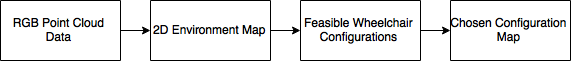
\includegraphics[width=3in]{figures/rgbdmap.png}
\caption{(TODO larger image) Pipeline for choosing a suitable parking spot.
The transition from point cloud data to a 2D environment map is described in
\autoref{sec:processingPointCloud} and \autoref{sec:2dmap}. Generating feasible configurations from the
environment map is described in \autoref{sec:feasibleparkingspot}. Selecting one
of the feasible configurations is described in
\autoref{sec:choosingparkingspot}.}
\label{fig:rgbdmap}
\end{figure}

\autoref{fig:rgbdmap} shows the general pipeline of the approach taken. The
point cloud data is transformed into a 2D environment map consisting of objects,
ground (free space), and unknown space. From this, the set of feasible
wheelchair configurations are determined, and a heuristic-based desirability
function is applied to choose an appropriate configuration from the feasible set.





% ====================
\subsection{Preprocessing the Point Cloud}
\label{sec:processingPointCloud}
% ====================
To make a map, we are inspired by the approaches of Holz \cite{holz2013towards}
and Gritti \cite{gritti2014kinect} to detect obstacles based on their height
from the ground plane. This allows detection of obstacles regardless of
their shape.

% One may argue: why not go directly from RGB-D sensor data to classification of
% parking spots, instead of a pipeline approach?
% First, we will see that ground detection is fairly robust and computationally
% cheap: there is very little error in this preprocessing step.
% Second, RGB-D data varies quite a bit; there is no clear mapping from RGB-D
% point clouds to location of parking spots. A learning approach would require an
% overbearing amount of training examples.

First, the point cloud is downsampled using a voxelized grid approach with a 5 cm
grid filter. This reduces the computational load and prevents excess weighting of
certain volumes in the upcoming ground plane detection.
Next, we estimate the parameters of a ground plane. 
The ground plane is needed for two reasons: it allows a 2D map to be easily
created aligned to the ground plane (\autoref{sec:2dmap}), and allows an
obstacle to be characterized by points above a certain distance above
the ground plane.
Multiple methods exist, including RANSAC \cite{fischler1981random}, the Hough
transform, and M-estimators \cite{holz2013towards}. We use a modified version
of RANSAC. 

Ground plane detection is done on each frame independently for robustness to
changing angles of the camera.
Algorithm \autoref{alg:modifiedRansac} shows the modified version of RANSAC.
Which ingests a point cloud $P$ of $n$ points in $\mathbb{R}^3$, and three
parameters: $k$, the number of iterations of testing a a new plane, $t$, the
threshold in metres in which points are considered part of the plane, and
$\theta_{max}$, the maximum inclination angle of possible ground planes.
Point cloud $P$ follows the format of a point cloud from an RGBD camera acquired
using the `openni2\_camera' package in ROS. This means the positive y-axis is
pointed roughly upwards in world coordinates, with the positive z-axis pointing
away from the camera along the horizontal plane of the camera.

The result is a ground plane represented as a 4-tuple $(a,b,c,d)$ satisfying
$ax + by + cz + d = 0$. Lines 7-9 highlight the additional constraint to avoid
detecting vertical planar surfaces (i.e. walls). Lines 16-18 ensure the ground
plane has a normal vector pointing upwards in the world space, standardizing any
ambiguity in defining a plane.

\begin{algorithm}
\caption{Modified RANSAC}
\label{alg:modifiedRansac}
\begin{algorithmic}[1]
\Require{
$k$ is the number of iterations to run, P are points in $\mathbb{R}^3$ with the
positive $y$ axis roughly vertical upwards, $\theta_{max}$ is the maximum
inclination angle, $t$ is the threshold used to identify if a point fits the
plane}
\Statex
\Function{ModifiedRANSAC}{$k, P, \theta_{max}, t$}
    \State $n \gets 3$, the minimum number of points to specify a plane
    \State $d \gets 0$, the number of points that lie on the current best plane
    \For{$k$ iterations}
        \State Draw a sample of $n$ non-collinear points from $P$ uniformly at random
        \State $l \gets$ the plane that includes all $n$ points
        \If{the angle between the x-z axis and plane $l$ is greater than $\theta_{max}$}
            \State the plane is too steep, continue to the next iteration
        \EndIf
        \State Find the subset of points $p \in P$ such that all points in $p$ are
        within distance $t$ from plane $l$
        \If{$|p| > d$}
            \State $bestPlane \gets l$, the current best ground plane candidate.
            \State $d \gets |p|$
        \EndIf
    \EndFor
    \If{the vector normal to $bestPlane$ has a negative $y$ coeficcient}
        \State flip the sign of the $y$ coefficient of $bestPlane$ 
    \EndIf
\EndFunction
\Statex
\Ensure{$bestPlane$, a 4-tuple $(a,b,c,d)$ that satisfies $ax + by + cz + d =
0$ representing the ground plane}
\end{algorithmic}
\end{algorithm}


We then rotate the point cloud $P$ to $P_{rotated}$ so the ground plane is
aligned with the x-y plane, the z-axis points upwards, the y-axis is the
direction the camera is facing, and the x-axis is chosen to complete the
right-handed reference frame. Doing so allows $P_{rotated}$ to be trivially
projected onto the ground plane.

\autoref{fig:pointclouds} shows an
example of the original point cloud $P$, where the positive z-axis is the
direction of depth from the camera, the y-axis points upwards in the world
frame, and the x-axis completes a right-handed reference frame. The detected
ground plane using Algorithm \ref{alg:modifiedRansac} is shown. The rotated
point cloud $P_{rotated}$ is shown on the right, with the ground plane aligned
with the x-y plane.

\begin{figure}
\centering
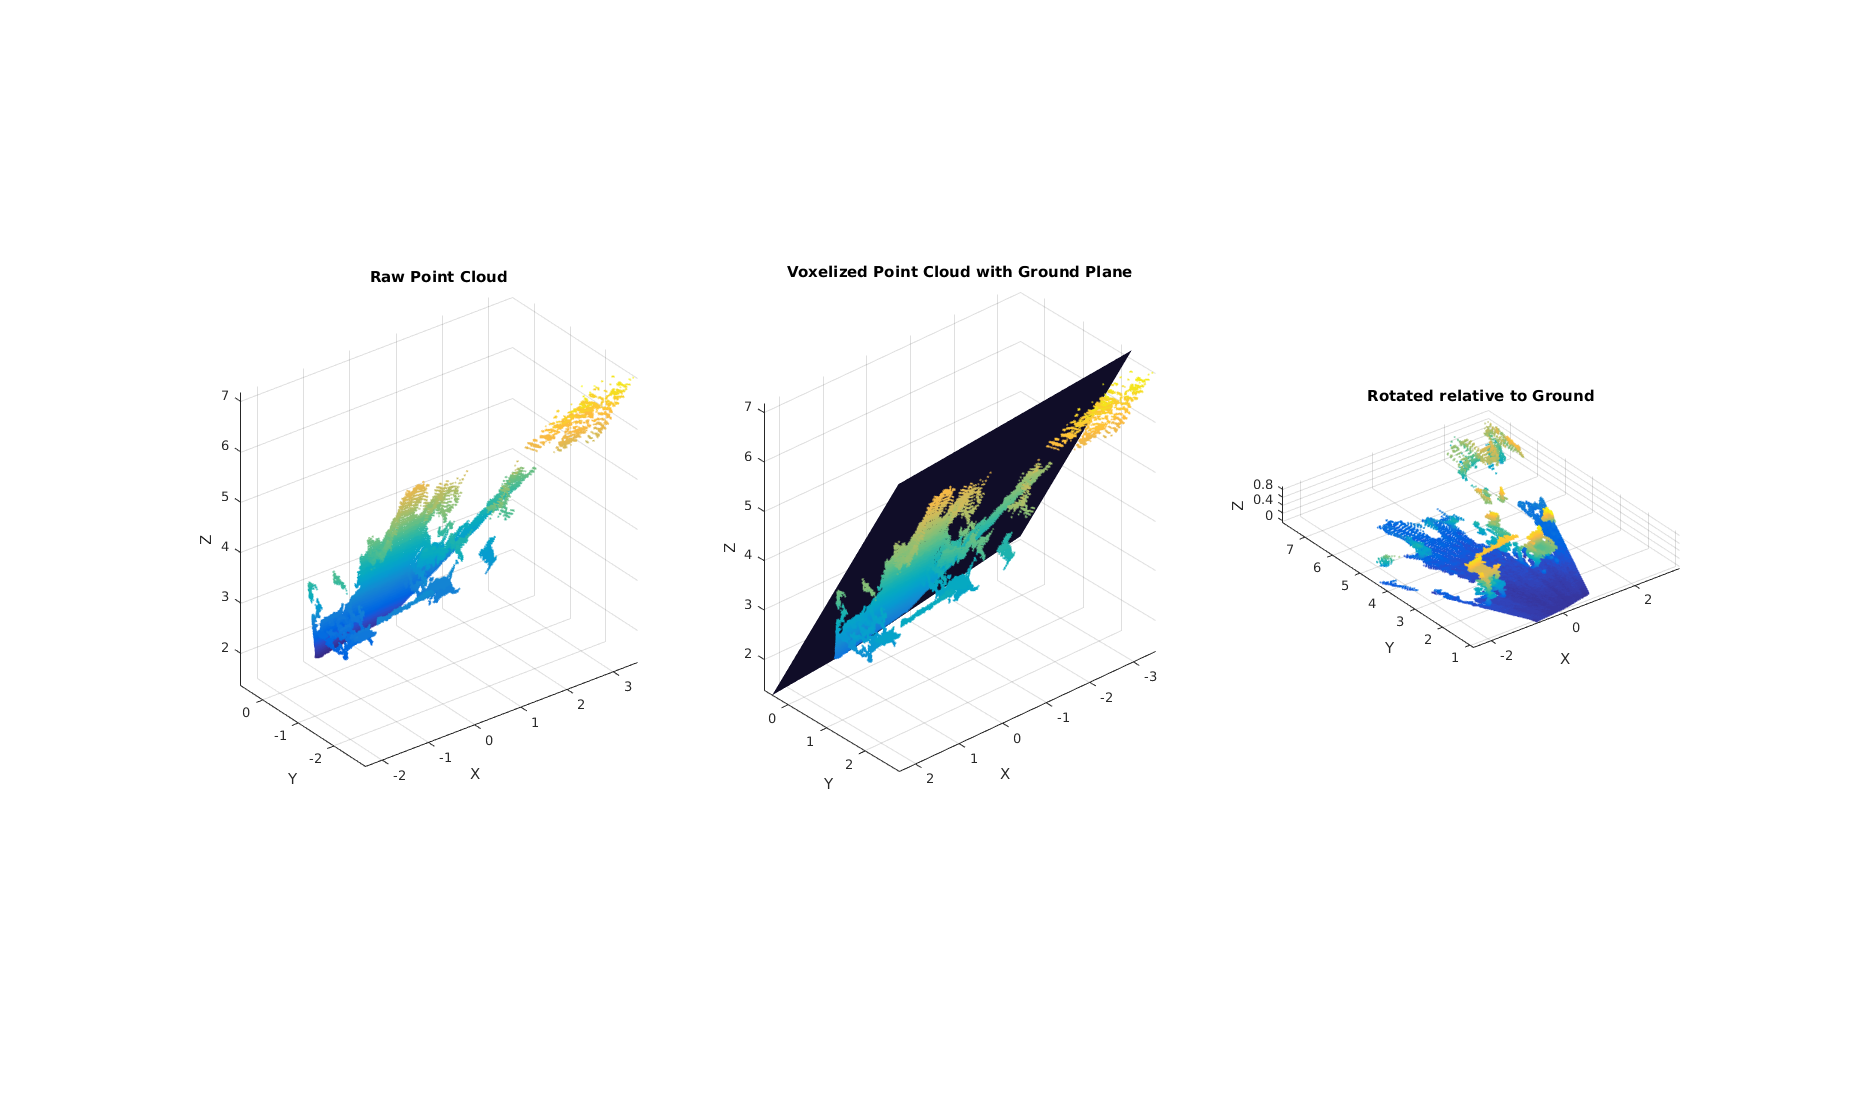
\includegraphics[width=6in]{figures/pointclouds.png}
\caption{Left: point cloud obtained from the RGBD sensor. Middle:
Downsampled point cloud with ground plane detected. Right: Rotated point cloud.}
\label{fig:pointclouds}
\end{figure}

% ====================
\subsection{Generating a 2D Map}
\label{sec:2dmap}
% ====================
We generate a 2D Map by projecting the 3D ground-aligned point cloud onto the
ground plane.
We classify each position on the 2D map as an object, the ground, or unknown.
Object and unknown classes are separated for use in
\autoref{sec:choosingparkingspot}.

Algorithm \autoref{alg:groundmapprojection} shows how the point cloud is
converted to a 2D map. It takes in the ground-aligned point cloud $P_{rotated}$
and two parameters: $gridStepSize$, a scalar in metres per pixel representing
the resolution of the map, and $groundThreshold$, the max height in metres that
a point can be considered part of the ground. This should be roughly the same
order of magnitude of $t$ from Algorithm \ref{alg:modifiedRansac}.

Let $p = (x_p, y_p, z_p) \in P_{rotated}$ be a of point in $\mathbb{R}^3$, with
$z_p$ representing the height above the ground for each point. Lines X to Y show
2D histograms are initialized to capture the location of ground and object
points. The histogram bounds are defined by taking the extremum points in both
the x and y dimensions.




A Gaussian blur with
a standard deviation of 0.7 is applied to filter out holes due to noise and
include a safety buffer. This is binarized on lines 12 and 13 by thresholding at
zero, resulting in a binary object map.
Similarly, the 2D ground histogram is binarized on lines 14 and 15 by first applying a Gaussian
blur with a standard deviation of 0.5 and thresholding at zero. 
Additionally, a 1m circle around the origin of the camera is assumed to be
viable positions in the ground map, which accounts for the minimimum range of
the RGBD camera. This is needed to ensure connectivity between the origin state
and farther feasible states, needed on line 2 in algorithm
\autoref{alg:feasibilitycheck}.

TODO talk about morphological dilation and erosion.

In a conservative fashion, any true pixels in the ground map that share a true
value in the object map is set to false, making the set of ground pixels and
object pixels mutually exclusive. 
% A third map is created for pixels that are not classified as a ground or object;
% hence each pixel must be classified as either on the ground plane, an object, or
% unknown.

\begin{algorithm}
\caption{TODO Ground Map Projection}
\label{alg:groundmapprojection}
\begin{algorithmic}[1]
\Require{$P_{rotated}$, $gridStepSize$, $groundThreshold$}
\Statex
\Function{GroundMapProjection}{$P_{rotated}, gridStepSize, groundThreshold$}
    \State $LB_x = \min_{p \in P_{rotated}}(x_p)$
    \State $UB_x = \max_{p \in P_{rotated}}(x_p)$
    \State $LB_y = \min_{p \in P_{rotated}}(y_p)$
    \State $UB_y = \max_{p \in P_{rotated}}(y_p)$
    \State $groundMap$, a 2D Histogram with bins spaced $gridStepSize$ metres apart
    \State $objectMap$, a 2D Histogram with bins spaced $gridStepSize$ metres apart
    \For{each point $p \in P_{rotated}$}
        \State $(x,y,z) \gets p$
        \If{$z < groundThreshold$}
            \State add $1$ to the appropriate $groundMap$ bin based on $(x,y)$
        \Else
            \State add $1$ to the appropriate $objectMap$ bin based on $(x,y)$
        \EndIf
    \EndFor
    \State $objectMap \gets GaussianBlur(objectMap, \sigma_1)$
    \State $objectMap \gets 1$ for each non-zero bin, $0$ otherwise

    \State $groundMap \gets GaussianBlur(groundMap, \sigma_2)$
    \State $groundMap \gets 0$ for each bin equal to zero and not already in $objectMap$, $1$ otherwise
\EndFunction
\Statex
\Ensure{$groundMap$, a 2D boolean array with values of $1$ representing the
ground, and $objectMap$}, a 2D boolean array with values of $1$ representing
impassible objects.
\end{algorithmic}
\end{algorithm}

\autoref{fig:groundobjectmap} shows an example of the resulting ground and
object map.

\begin{figure}
\centering
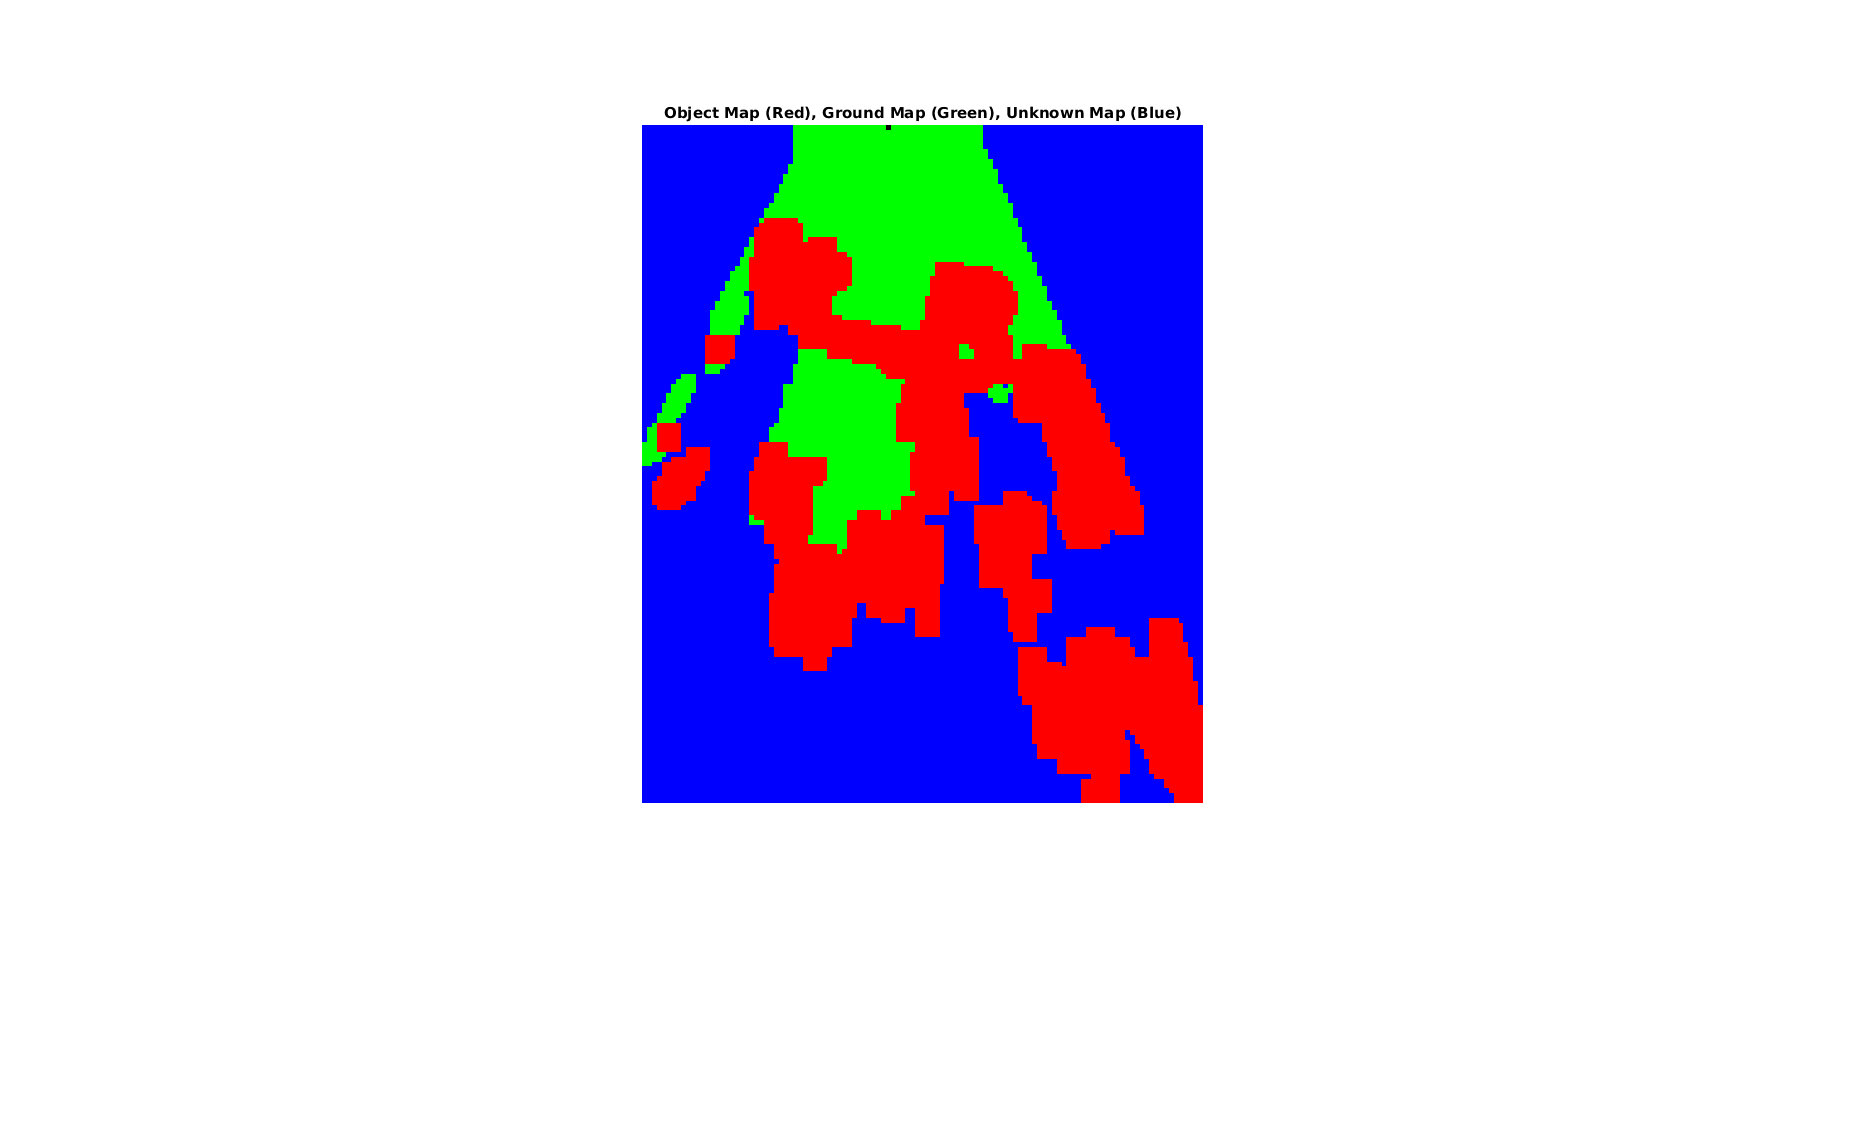
\includegraphics[width=5in]{figures/groundobjectmap.png}
\caption{2D projection of the point cloud. Green (light gray on black and white)
is classified as ground, red (medium gray) is classified as objects, and blue
(dark gray) is classified as unknown, determined by Algorithm
\autoref{alg:groundmapprojection}. The black pixel near the centre top
represents the location of the wheelchair during time of capture.}
\label{fig:groundobjectmap}
\end{figure}

% --------------------
\section{Motion Planning}
% --------------------

% --------------------
\subsection{Introduction to Motion Planning}
% --------------------
An in-depth introduction can be found in Chapter 1.3 of Lavalle
\cite{lavalle2006planning}.
% \begin{itemize}
% \item State
% \item Time
% \item Actions
% \item Initial and Goal States
% \item Feasibility and Optimality Criterion
% \item A Plan
% \end{itemize}

% --------------------
\subsection{Simple Motion Planning}
% --------------------
The simplest motion planning problems assume knowledge of a global map, a fixed
known goal state and a fixed known initial state. The problem is to determine a
feasible path from the initial state to the goal state. An optimality criterion
may also be applied to choose the best path if multiple feasible ones are found.

Notably, two important concepts are ignored in determining the path:
differential constraints of the system and the use of feedback. Differential
constraints refer to how states transition to other states, and is inherent in
real-world systems, eg. a system's dynamics. For example, a car can easily move
fowards and backwards, but cannot immediately move side to side, which may be
assumed when determining a path. Feedback refers to the technique of refining
further actions based on newly sensed data. In simulations feedback may not be
necessary, but in real-world systems, errors in sensing and modeling build up
over time without it.

In this simple case, the solution involves a generated path that is followed in
an open-loop manner, or if subject to real-world constraints (see
\autoref{fig:lavalle2006planning119}), the generated path is smoothed to obey
the system's dynamics and feedback is used to closely follow the path. "Notably
this approach is highly decoupled as feedback and dynamics are neglected in
constructing the original path" \cite{lavalle2006planning}. The smooth path may
now obey the robot's dynamics, but may no longer be feasible. Feedback is used
as an inefficient afterthought to stay on a track that itself may not be
feasible or optimal.

\begin{figure}
\centering
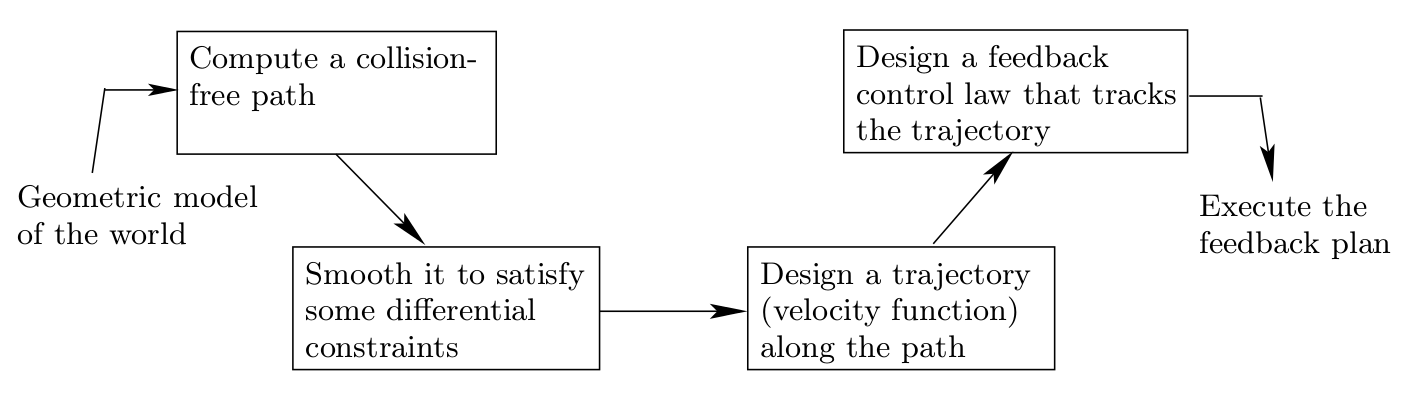
\includegraphics[width=3in]{figures/lavalle2006planning119.png}
\caption{From \cite{lavalle2006planning}. A refinement approach that has been
used for decades in robotics. Note the initial path is computed without
consideration of differential constraints or the use of feedback}
\label{fig:lavalle2006planning119}
\end{figure}

Even in this simple case, obtaining an optimal or even feasible path is not
straightforward if the state space is large. A* search for trivially sized state
spaces and sampling-based techniques such as RRTs (RRT* for optimality) and PRMs
have proven to be the methods of choice (citation?), though it is still an
ongoing field of interest (cite 2015 RRT/PRM papers).

The ROS Navigaiton Stack
(\url{http://www.dis.uniroma1.it/~nardi/Didattica/CAI/matdid/robot-programming-ROS-introduction-to-navigation.pdf})
is an example of this.
% --------------------
\subsection{Feedback Motion Planning}
% --------------------
Incorporating feedback directly when generating a path is a secondary option. 
For a full description of feedback motion planning, see Chapter 8 of Lavalle
\cite{lavalle2006planning}.
In the back-in parking problem, the trajectory to the goal state is assumed
visible, and hence generating a vector field may be suitable. A reliable model
and odometry data, however, varies from wheelchair to wheelchair, and so the
solution must be robust to model inaccuracies.

Two approaches can be taken: One, a target parking spot can be determined from
the initial position of the wheelchair, and the initial point cloud can be used
as a local map. The task is then to simultaneously localize the wheelchair's
position in the initial map while following a trajectory towards the parking
spot. This is visualized in \autoref{fig:determinedrive2}.
 
\begin{figure} % --------------------------------------
\centering
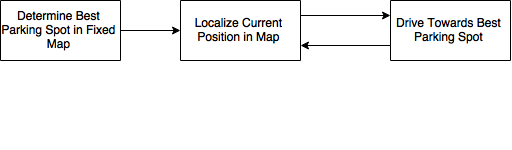
\includegraphics[width=3in]{figures/determinedrive2.png}
\caption{Feedback loop with a fixed goal state and map}
\label{fig:determinedrive2}
\end{figure}   % --------------------------------------

A second approach is to instead continuously update the initial map with new
sensor data, in effect performing SLAM on a constrained trajectory. The goal
state can then also be continously updated as new map information is ingested,
and the trajectory of the wheelchair will be updated based on this.
\autoref{fig:determinedrive1} illustrates this.
 
\begin{figure} % --------------------------------------
\centering
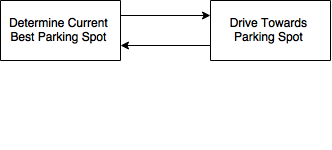
\includegraphics[width=3in]{figures/determinedrive1.png}
\caption{Feedback loop}
\label{fig:determinedrive1}
\end{figure}   % --------------------------------------

% ====================
\section{Related Work}
\label{sec:backinginlitreview}
% ====================
One way is to have a fixed, open-loop trajectory. This method is very old and
has been done for cars.

\cite{sermeno2006vision} uses vision-based PID control (page 17)

Angus's paper using PID

\subsection{Real-time Motion Planning}

From \cite{hauser2013recognition}:
Sampling-based motion planners such as Probabilistic Roadmaps (PRMs) and
Rapidly-Exploring Random Trees (RRTs) are effective at planning collision-free
motion for high-dimensional robot systems ( LaValle 2006), and have also been
successfully applied to hard real-time planing for 2D helicopters ( Frazzoli et
al. 2002) and ground vehicles ( Petti and Fraichard 2005). Recently they have
been applied to teleoperation interfaces for robot manipulator arms ( Hauser
2011). But these works have traditionally focused on finding feasible paths
rather than optimal ones.  Sampling-based approaches have been recently
developed for the optimal motion planning problem ( Karaman and Frazzoli 2010),
but they have not yet been applied to time- varying cost functions and moreover
converge too slowly for real-time use. An alternative approach is numerical
opti- mization over a trajectory parameterization ( Bobrow et al.  2001).
Optimization approaches can achieve optimality with a fast convergence rate,
albeit only locally. Our hybrid plan- ner combines the strength of
sampling-based and numeri- cal approaches and is designed specifically to
produce high- quality paths quickly for a broad class of cost functions.

% ====================
\section{Visual Odometry}
% ====================
Pictures of sequences

% ====================
\section{Pure Pursuit Path Planner}
% ====================

% ====================
\section{Results}
% ====================
Qualtitative Pictures.

Time to reach.

% 
% % --------------------
% \section{Practical Options}
% % --------------------
% 
% \begin{figure}
% \centering
% 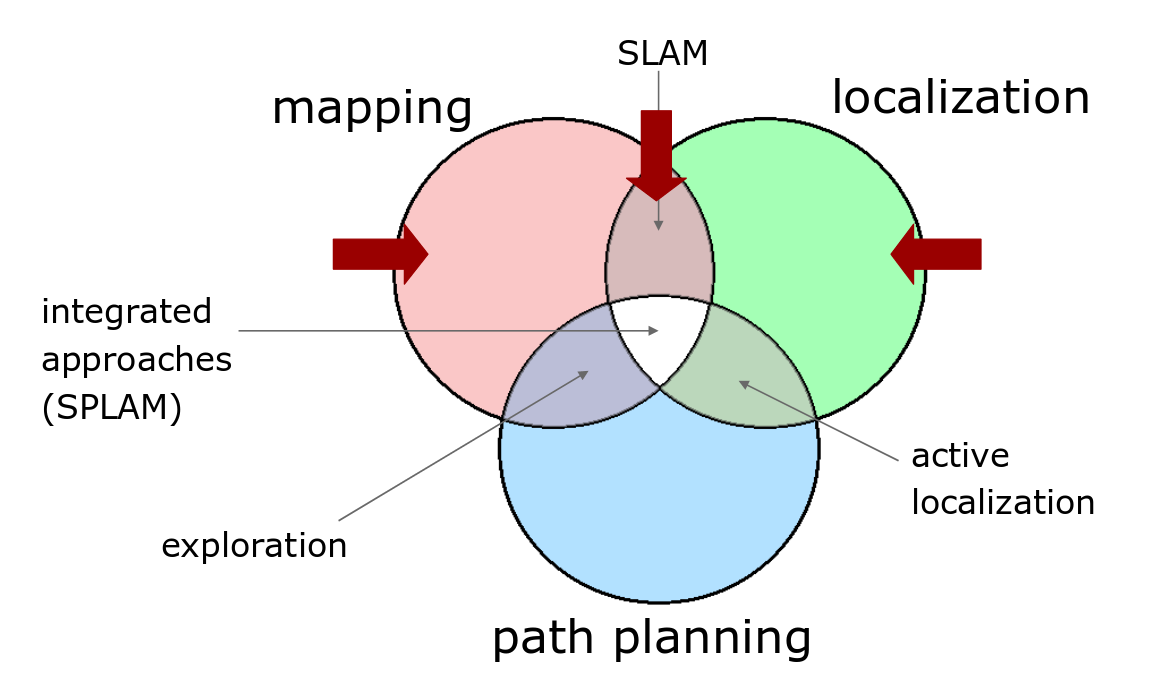
\includegraphics[width=3in]{figures/mappinglocalizationpathplanningvenndiagram.png}
% \caption{Venn Diagram of Localization, Mapping and Path Planning}
% \label{fig:mappinglocalizationpathplanningvenndiagram}
% \end{figure}

% --------------------

% --------------------
\chapter{Experiments}
\label{ch:experiments}


% ====================
\section{Installing F}
% ====================

\begin{enumerate}
	\item implement princeton RGBD algorithm
	\item implement struck
	\item implement 2014 color tracking algorithm
	\item implemenmt Gaussian processes algorithm
\end{enumerate}

\subsubsection{Implementing the princeton "song2013tracking" RBGD algorith}

code is in song2013tracking. 

% --------------------



%\include{model}
%\include{impl}
%\include{discussion}
%\include{conclusions}

%    3. Notes
%    4. Footnotes

% --------------------
%    5. Bibliography
% --------------------
\begin{singlespace}
\raggedright
\bibliographystyle{abbrvnat}
\bibliography{biblio}
\end{singlespace}

% --------------------
\appendix
%    6. Appendices (including copies of all required UBC Research
%       Ethics Board's Certificates of Approval)
%\include{reb-coa}	% pdfpages is useful here
% --------------------
% \chapter{Supporting Materials}

This would be any supporting material not central to the dissertation.
For example:
\begin{itemize}
\item additional details of methodology and/or data;
\item diagrams of specialized equipment developed.;
\item copies of questionnaires and survey instruments.
\end{itemize}


% --------------------
\backmatter
%    7. Index
% See the makeindex package: the following page provides a quick overview
% <http://www.image.ufl.edu/help/latex/latex_indexes.shtml>
% --------------------


\end{document}
